\documentclass[a4paper,10pt]{article}
	 \textheight = 24cm
	 \textwidth = 18cm
	 \topmargin = -1cm
	 \oddsidemargin = -1cm
	 
\setcounter{part}{0} 	
\setcounter{secnumdepth}{3} % Para enumerar hasta subsubsection
\setcounter{tocdepth}{3} % Para enumerar hasta subsubsection 
 
\usepackage[utf8]{inputenc}
\usepackage[none]{hyphenat} %Paquete para indicar que no separe las palabras
\usepackage{graphicx} %Paquete para incluir imágenes
\usepackage{fancyhdr} %Paquete para modificar los pies de página y encabezados
\usepackage[hidelinks]{hyperref} 
\usepackage{enumitem}
\usepackage{hyperref}

\usepackage{listings} %Paquete para poner código de programación


\lstset{frame=tb,
  language=C,
  aboveskip=3mm,
  belowskip=3mm,
  showstringspaces=false,
  columns=flexible,
  basicstyle={\small\ttfamily},
  numbers=left,
  numberstyle=\tiny\color{gray},
  keywordstyle=\color{blue},
  commentstyle=\color{dkgreen},
  stringstyle=\color{mauve},
  breaklines=true,
  breakatwhitespace=true,
  tabsize=3
}

\renewcommand{\refname}{Bibliografía}
\renewcommand{\appendixname}{Apéndices}
\renewcommand{\contentsname}{Índice}
\renewcommand{\thesection}{\arabic{section}}

\begin{document}
%--------------------------------------------------------------------
\thispagestyle{empty}
\begin{figure}[h]

\includegraphics[scale=0.4]{images/logo-umu.jpg} \hspace{100mm}

\includegraphics[scale=0.2]{images/logo-fium.png}
\centering
\end{figure}

\vspace{15mm}

\begin{center}
\rule{100mm}{0.1mm} \\
\vspace{5mm}
\begin{Huge}
 \textbf{Universidad de Murcia}\\ \vspace{10mm}
\end{Huge}
\begin{huge}
 \textbf{Facultad de Informática}
\end{huge}
\vspace{5mm} \\
\rule{100mm}{0.5mm}

\vspace{20mm}

\begin{Huge}
 IA para el Desarrollo de Videojuegos \\ \vspace{5mm}
\end{Huge}

\begin{LARGE}
 Real Time Wargame
\end{LARGE}

\vspace{15mm}

\begin{Large}
 \textbf{Autores} \\ \vspace{2mm}
 Antonio López Martínez-Carrasco\\ \vspace{2mm}
 \textit{antonio.lopez31@um.es} \\ \vspace{4mm}
 José María Sánchez Salas\\ \vspace{2mm}
 \textit{josemaria.sanchez12@um.es}
\end{Large}

\vspace{7mm}

\begin{Large}
 \textbf{Profesores} \\ \vspace{2mm}
 Francisco Javier Martín-Blázquez Gómez \\ \vspace{2mm}
 \textit{jgmarin@um.es} \\ \vspace{4mm}
 Luis Daniel Hernández Molinero \\ \vspace{2mm}
 \textit{ldaniel@um.es}
\end{Large}
\end{center}
%--------------------------------------------------------------------
%--------------------------------------------------------------------
\newpage
\pagestyle{fancy}
\renewcommand{\headrulewidth}{0.5pt} %Definimos el grosor de la línea
\lhead[IA para el Desarrollo de Videojuegos]{IA para el Desarrollo de Videojuegos}
\rhead[Real Time Wargame]{Real Time Wargame}
\renewcommand{\footrulewidth}{0.5pt}
\tableofcontents
\newpage


\part{Introducción y estructura de la aplicación}
%--------------------------------------------------------------------
\medskip
\section{Introducción}
Este documento corresponde con la documentación del proyecto Real Time Wargame propuesto por la asignatura IA para el Desarrollo de Videojuegos perteneciente a la mención de Computación del 4º curso del Grado de Ingeniería Informática impartida por la Universidad de Murcia. \\

El proyecto consiste en implementar algunos elementos de inteligencia artificial en un entorno de juego de guerra en tiempo real. Estos elementos de inteligencia artificial van desde la parte reactiva, como comportamientos más básicos, como puede ser moverse de un sitio a otro, hasta la parte táctica, como comportamientos tácticos basados en una máquina de estados. \\

Para la implementación de este proyecto, hemos decidido utilizar la librería gráfica LibGDX \cite{libgdx}. El motivo por el cuál nos hemos decantado por esta librería es porque es una librería sin licencia, implementada en Java, con muy buena documentación y que no requiere de un hardware específico para su ejecución, además de que estamos muy acostumbrados a trabajar en Java. Así pues, no hemos implementado este proyecto para ningún hardware específico, simplemente hemos hecho uso del IDE Eclipse junto con la librería LibGDX, programando y ejecutándolo en nuestros respectivos ordenadores. \\

Este documento consta de ocho partes fundamentales: la primera de ellas se encarga de introducir el proyecto, así como también la estructura que tiene el proyecto desarrollado en Java. La segunda contiene un breve manual de uso para los usuarios. La tercera contiene la explicación de la clase principal del programa, el mapa implementado y la interacción con el usuario. La cuarta parte comenta toda la parte de la inteligencia artificial reactiva que hemos implementado, así como el modelo de objetos del videojuego que hemos desarrollado. La quinta trata las diversas implementaciones del Pathfinding que hemos llevado a cabo. La sexta parte contiene la parte de la inteligencia artificial táctica que hemos implementado, así como las modificaciones que hemos llevado a cabo en el modelo mencionado en la sección cuarta para poder introducir la parte táctica al modelo. La séptima parte comenta la implementación que se ha llevado a cabo del Flocking pedido en el proyecto. Y por último, en la parte octava, se hace una recopilación de todos los elementos opcionales que hemos implementado. \\

Las dos últimas partes de este documento constan de las conclusiones que hemos obtenido tras la realización de este proyecto y la bibliografía consultada para el mismo.



%--------------------------------------------------------------------
\medskip
\section{Estructura de la aplicación}
La estructura que hemos llevado a cabo en este proyecto ha sido una estructura en paquetes (típica estructura de cualquier proyecto en Java). Esta estructura es la siguiente:
\begin{itemize}
 \item Primero se encuentra el paquete \texttt{com.mygdx.iadevproject} que contiene la clase principal del proyecto, así como la clase que crea todos los personajes del videojuego.
 \item Seguidamente se encuentra el paquete \texttt{com.mygdx.iadevproject.aiReactive} que contiene toda la parte reactiva de la inteligencia artificial: desde los comportamientos no acelerados, pasando por los comportamientos acelerados, delegados y de grupo; los árbitros y el pathfinding. Cada uno de estos elementos, se encuentra en su paquete correspondiente.
 \item El paquete \texttt{com.mygdx.iadevproject.aiTactical} contiene toda la parte táctica de la inteligencia artificial: los roles implementados, los estados de las máquinas de estados implementadas, así como los nodos del árbol de decisión implementado.
 \item El paquete \texttt{com.mygdx.iadevproject.model} contiene todo el modelo de objetos que hemos considerado para este proyecto.
 \item El paquete \texttt{com.mygdx.iadevproject.map} contiene todo lo referente a la creación del mapa, así como a partir de él, la inicialización de los grids necesarios para el pathfinding.
 \item El paquete \texttt{com.mygdx.iadevproject.mapOfInfluence} contiene la parte del cálculo de los mapas de influencia. Así como su visualización.
 \item El paquete \texttt{com.mygdx.iadevproject.userInteraction} encapsula la interacción del sistema con el usuario.
 \item Y por ultimo, el paquete \texttt{com.mygdx.iadevproject.waypoints} encapsula toda la creación y manejo de los waypoints del juego.
\end{itemize}

Para poder probar el correcto funcionamiento todas las funcionalidades implementadas, se ha creado una carpeta de test que tiene la misma estructura que la carpeta de fuentes, y que contiene todos los test implementados de toda la funcionalidad del sistema: comportamientos, árbitros, pathfinding, roles, formaciones, etc.


\part{Clase principal y mapa}
%--------------------------------------------------------------------
\medskip
\section{Clase principal}
Todo lo referente a esta sección, se encuentra dentro del paquete \texttt{com.mygdx.iadevproject} del proyecto. La clase principal de nuestro proyecto es la clase \texttt{IADeVProject} y es la que contiene los siguientes elementos:
\begin{itemize}
 \item \textbf{Constantes}. Estas son: el tamaño del mapa (alto y ancho); el tamaño de las celdas de los grids, así como el tamaño de estos (alto y ancho); valores de infinito, coste y terreno por defecto; y el tamaño de los objetos del mundo (alto y ancho, obtenidos a partir de la información del mapa).
 \item \textbf{Mapas}. Estos son: el mapa real que se dibuja; el mapa de costes para el PathFinding; el mapa de terrenos para modificar la velocidad de un personaje dependiendo del terreno por donde se mueve (exceptuando el mapa real, todos los demás son los que se denominan grids y todos tienen el mismo tamaño).
 \item \textbf{Variables globales}. Estas son: los objetos y obstáculos del mundo; el conjunto de objetos seleccionados por el usuario (utilizando el ratón); la cámara; el flag que indica si se dibujan, o no, las líneas de depuración de los distintos comportamientos; así como las variables necesarias para que desde los comportamientos se puedan dibujar las líneas de depuración. También están las bases y manantiales de los equipos, el controlador de la interacción con el usuario, las variables que indican si se pausa (o no) el juego y si se dibuja (o no) el mapa de influencia encima del mapa real, así como las variables que indican qué equipo ha ganado (si lo hay) y la variable que indica si puede haber (o no) ganador en la partida.
\end{itemize}

Esta clase se encarga de crear e inicializar todos los elementos anteriores, de renderizar el seguimiento del juego y, una vez terminado, eliminar todos los elementos creados para el renderizado. Para la creación de todos los personajes, se ha creado la clase \texttt{CreateCharacters} que proporciona un único método estático \texttt{createCharacters()}. También se encarga de inicializar los waypoints del juego, así como los mapas de influencia. Para esto, hace uso de los métodos estáticos proporcionados por las clases \texttt{Waypoints} y \texttt{SimpleMapOfInfluence} (véase secciones \ref{waypoints} y \ref{mapas-influencia}).\\

El control de la interacción del usuario con el juego se ha implementado en la clase \texttt{InputProcessorIADeVProject} (ver sección \ref{interaccion}), que contiene todos los manejadores para las posibles acciones que puede realizar el usuario con el teclado y el ratón. Debido a que el usuario puede seleccionar objetos del mundo, cuando se realiza la selección para que añadan los objetos al conjunto de objetos seleccionados, se hace uso del método \texttt{addToSelectedObjectsList()} de la clase \texttt{IADeVProject}. Como también se proporciona la funcionalidad de eliminar la selección de objetos, dicha clase también proporciona el método \texttt{clearSelectedObjectsList()}. \\

Debido a que el tamaño de los distintos grids y el tamaño del mapa pueden no ser iguales (pues depende del tamaño de las celdas), es necesario hacer una conversión entre las posiciones reales del mapa y las posiciones correspondientes del grid. Por eso mismo, la clase \texttt{IADeVProject} proporciona los dos siguientes métodos:
\begin{itemize}
 \item \texttt{mapPositionTOgridPosition() y gridPositionTOmapPosition()}. Ambos reciben como parámetros el tamaño de la celda del grid y un vector con la posición que se quiere convertir. El primero transforma una posición del mapa a una posición del grid (índices de la matriz que representa al grid), y el segundo hace la inversa: transforma una posición del grid a una posición del mapa.
\end{itemize}

También proporciona métodos para obtener las bases y manantiales de cada equipo, así como la posición de ambas.



%--------------------------------------------------------------------
\medskip
\section{Mapa}
Todo lo referente a esta sección, se encuentra dentro del paquete \texttt{com.mygdx.iadevproject.map} del proyecto. El mapa que se ha diseñado para este proyecto se muestra en la Figura \ref{mapa:mapa}.
\begin{figure}[!th]
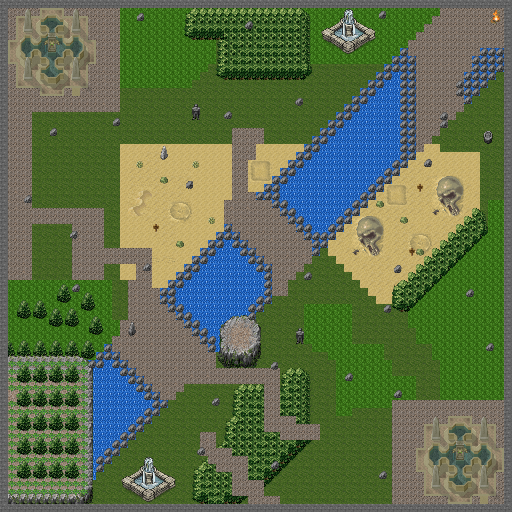
\includegraphics[scale=0.6]{map}
\centering
\caption{Mapa diseñado para el proyecto.}
\label{mapa:mapa}
\end{figure}

Como se puede observar, existen seis tipos de terrenos:
\begin{itemize}
 \item \textbf{Agua y montañas}. Representan los terrenos infranqueables. Como indica el enunciado del proyecto, los dos países se encuentran separados por un río con tres puentes para cruzarlo.
 \item \textbf{Desierto y bosque}. Se identifican de manera directa en el mapa. También se tiene como bosque los árboles que se encuentran dentro la pradera situada en la parte inferior izquierda del mapa.
 \item \textbf{Pradera}. Se corresponde con los tramos de color verde más claro.
 \item \textbf{Sendero}. Se corresponde con el fondo del mapa.
 \item \textbf{Camino}. Se corresponde con los tramos de color gris. Las bases de los países se encuentran encima de este tipo de terreno.
\end{itemize}

Para representar los terrenos en el proyecto, se ha implementado el enumerado \texttt{Ground} que proporciona los siguientes métodos:
\begin{itemize}
 \item \texttt{getCost()}. Debido a que cada terreno tiene un coste asociado, este método devuelve dicho coste.
 \item \texttt{getGround(int cost)}. Se trata de un método estático que dado un coste, devuelve el terreno al que pertenece. Si el coste que se pasa como argumento no se corresponde con ningún terreno, devuelve \texttt{null}.
\end{itemize}

También podemos observar que cada uno de los equipos tiene un manantial donde los personajes pueden curarse y a donde van cuando estos mueren. \\

Para diseñar el mapa, se ha hecho uso de la herramienta \texttt{Tiled Map Editor} \cite{tiledMap} que proporciona una sencilla forma de diseñar mapas por capas, permitiendo que puedas crear capas de distintos tipos (de tiles, de objetos, etc), lo que nos facilita la creación e inicialización de los distintos grids que utilizamos. Lógicamente, las capas que se encuentran en el mapa, se corresponden con los distintos tipos de terrenos mencionados anteriormente (excluyendo la capa de objetos). \\

Para introducir el mapa diseñado en el proyecto, \texttt{LibGDX} nos proporciona la clase \texttt{TiledMap}. Sin embargo, esta clase, a la hora de renderizar, si existe alguna capa de objetos por defecto, no la dibuja. Por este motivo, implementamos la clase \texttt{TiledMapIADeVProject}, que sobreescribe los métodos de renderizado para que se dibujen las capas de objetos. \\

Una vez que tenemos el mapa diseñado e introducido en nuestro proyecto, hay que inicializar los distintos grids en correspondencia con dicho mapa. Para ello, está la clase \texttt{MapsCreatorIADeVProject}, que proporciona un único método estático \texttt{createMaps()} y que se encarga de recorrer, para cada terreno, su capa correspondiente e inicializar los grids a los valores correspondientes.





























\part{IA reactiva}
%--------------------------------------------------------------------
\medskip
\section{Steerings}
\label{steerings}

%--------------------------------------------------------------------
\medskip
\section{Comportamientos}
Todo lo referente a esta sección, se encuentra dentro del paquete \texttt{com.mygdx.iadevproject.aiReactive.behaviour} del proyecto. Para generalizar el uso de los comportamientos, se ha decidido crear la interfaz \texttt{Behaviour} que tienen que implementar todos los distintos tipos de comportamientos. Esta interfaz proporciona un solo método:
\begin{itemize}
 \item \texttt{getSteering()}, que no recibe ningún parámetro y devuelve un \texttt{Steering}. Este método no recibe ningún parámetro para generalizar los comportamientos, pues no todos los comportamientos necesitan lo mismo para poder calcular su steering. De esta manera, en la creación del comportamiento concreto, se ha de proporcionar todos los datos necesarios para que él pueda calcular su steering, implementando a su manera, este método. 
\end{itemize}

A continuación, en las siguientes subsecciones se muestran todos los comportamientos que hemos implementado.

%--------------------------------------------------------------------
\medskip
\subsection{Comportamientos no acelerados}
Todo lo referente a esta sección, se encuentra dentro del paquete \\ \texttt{com.mygdx.iadevproject.aiReactive.behaviour.noAcceleratedUnifMov} del proyecto. Los distintos comportamientos no acelerados que hemos implementado son:
\begin{itemize}
 \item \texttt{Arrive\_NoAccelerated}. Este comportamiento consiste en llegar hacia un objetivo, rodeado por un radio de satisfacción en el que se supone que el personaje ya ha llegado, a la máxima velocidad y en un tiempo determinado. Así, para la creación de este comportamiento, son necesarios los siguientes parámetros:
 \begin{itemize}
  \item El personaje que va a aplicar el comportamiento.
  \item El objetivo al que se quiere dirigir.
  \item La máxima velocidad con la que se aplica el comportamiento.
  \item El radio de satisfacción.
  \item El tiempo que se tarda en llegar al objetivo.
 \end{itemize}
 
 \item \texttt{Flee\_NoAccelerated}. Este comportamiento consiste en alejarse de un determinado objetivo, a la máxima velocidad. Para la creación de este comportamiento, son necesarios los siguientes parámetros:
 \begin{itemize}
  \item El personaje que va a aplicar el comportamiento.
  \item El objetivo del que se quiere alejar.
  \item La máxima velocidad con la que se aplica el comportamiento.
 \end{itemize}
 
 \item \texttt{Seek\_NoAccelerated}. Este comportamiento es el opuesto al anterior, consiste en ir hacia un determinado objetivo, a la máxima velocidad. Los parámetros son los mismos que los necesarios en el anterior. 
 
 \item \texttt{Wander\_NoAccelerated}. Este comportamiento consiste en moverse de manera aleatoria, con un ángulo máximo de rotación a la máxima velocidad. Para la creación de este comportamiento, son necesarios los siguientes parámetros:
 \begin{itemize}
  \item El personaje que va a aplicar el comportamiento.
  \item La máxima velocidad con la que se aplica el comportamiento.
  \item El máximo ángulo de rotación que puede cambiar un personaje su orientación.
 \end{itemize}
\end{itemize}

Es importante destacar, que estos cuatro comportamientos, dentro del método \texttt{getSteering()} modifican la orientación del personaje.


%--------------------------------------------------------------------
\medskip
\subsection{Comportamientos acelerados}
Todo lo referente a esta sección, se encuentra dentro del paquete \\ \texttt{com.mygdx.iadevproject.aiReactive.behaviour.acceleratedUnifMov} del proyecto. Los distintos comportamientos acelerados que hemos implementado son:
\begin{itemize}
 \item \texttt{Align\_Accelerated}. Este comportamiento consiste en adoptar la misma orientación que otro personaje (personaje destino) mediante un movimiento giratorio. La condición principal para llevar a cabo dicho movimiento es que debemos girar hacía el lado cuyo ángulo hacia la orientación destino sea menor. Además, en función de lo cerca que esté la fuente del destino (del valor del ángulo diferencia), la fuente se comportará del manera distinta. Hasta llegar a un ángulo exterior, la fuente gira con la máxima velocidad angular permitida. Al superar dicho ángulo, el personaje va adaptando su velocidad angular. Cuando se supera un ángulo interior, se devuelve un steering con aceleración lineal nulo y con aceleración angular inversa a la velocidad angular del personaje fuente. Para crear este comportamiento son necesarios los siguientes parámetro:
 \begin{itemize}
 	\item Personaje origen y \texttt{WorldObject} destino.
 	\item Máxima aceleración angular que el personaje puede aplicar.
 	\item Máxima rotación (velocidad angular) que el personaje puede aplicar.
 	\item \texttt{targetRadious} del personaje destino (ángulo interior). En este comportamiento no es un radio, sino un ángulo.
 	\item \texttt{slowRadious} del personaje destino (ángulo exterior). En este comportamiento no es un radio, sino un ángulo.
 	\item \texttt{timeToTarget} es el tiempo que queremos que tarde el personaje en realizar este comportamiento.
 \end{itemize}
 \item \texttt{AntiAlign\_Accelerated}. Este comportamiento consiste en adoptar la orientación opuesta de un personaje destino mediante un movimiento giratorio. Al igual que antes, debemos girar hacía el lado cuyo ángulo hacia la orientación deseada sea menor. El funcionamiento del comportamiento es igual que el anterior (aunque en este caso, debemos posicionarnos con orientación inversa a la del destino). Para crear este comportamiento son necesarios los mismos parámetros que el comportamiento anterior.
 \item \texttt{Arrive\_Accelerated}. En este comportamiento se definen 3 zonas distintas en las que el comportamiento del personaje es distinto. Podemos encontrar 2 radios ficticios con respecto al personaje destino. En primer lugar, el personaje fuente va aplicando la máxima aceleración establecida hasta llegar al radio exterior. Al llegar al radio exterior, el personaje adapta su velocidad en función de la distancia entre el personaje destino y él, hasta llegar al radio interior. Finalmente, cuando el personaje esta en el radio interior, este comportamiento devuelve el steering nulo (con valor 0). Para crear este comportamiento son necesarios los siguientes parámetro:
 \begin{itemize}
 	\item Personaje origen y \texttt{WorldObject} destino.
 	\item El valor de la máxima aceleración permitida.
 	\item El valor de la máxima velocidad permitida.
 	\item \texttt{targetRadious}. El radio de la circunferencia ficticia interior.
 	\item \texttt{slowRadious}. El radio de la circunferencia ficticia exterior.
 	\item \texttt{timeToTarget} es el tiempo que queremos que tarde el personaje en realizar este comportamiento.
 \end{itemize}
 \item \texttt{Arrive\_Accelerated\_WithOneRadius}. Este comportamiento es una mezcla entre un Seek y un Arrive (hereda del comportamiento Seek Acelerado). En este comportamiento podemos encontrar solamente un radio ficticio alrededor del personaje destino. La fuente se mueve aplicando un comportamiento Seek Acelerado normal hasta llegar al radio y cuando entra en él empieza a frenar (devolviendo un steering cuyo vector aceleración tiene un sentido contrario al vector velocidad del personaje fuente). A parte de los parámetros del padre (comportamiento Seek), también son necesarios los siguientes parámetros:
 \begin{itemize}
 	\item \texttt{targetRadious}. El radio de la circunferencia ficticia.
 \end{itemize}
 \item \texttt{Flee\_Accelerated}. Cuando un personaje aplica este comportamiento, se aleja del personaje destino aplicando la máxima aceleración establecida. Para crear este comportamiento son necesarios los siguientes parámetro:
 \begin{itemize}
 	\item El personaje que va a aplicar el comportamiento.
  	\item El objetivo al que se quiere dirigir.
  	\item La máxima aceleración con la que se aplica el comportamiento.
 \end{itemize} 
 \item \texttt{Seek\_Accelerated}. Este comportamiento consiste en ir hacia un punto objetivo a la máxima aceleración posible. Para la creación de este comportamiento, son necesarios los siguientes parámetros:
 \begin{itemize}
  \item El personaje que va a aplicar el comportamiento.
  \item El objetivo al que se quiere dirigir.
  \item La máxima aceleración con la que se aplica el comportamiento.
 \end{itemize}
 Para este comportamiento, se ha hecho uso de las dos implementaciones que nos han proporcionado los profesores en la teoría: la implementación de Millington y la implementación de Reynolds. De esta manera, por defecto, se utiliza la implementación de Millington, pero si se quiere cambiar de implementación, proporciona el método \texttt{setMode()} que recibe como parámetro el modo al que se quiere cambiar. El valor del modo de cada una de las implementaciónes está en las constantes \texttt{SEEK\_ACCELERATED\_MILLINGTON} y \texttt{SEEK\_ACCELERATED\_REYNOLDS} correspondientemente.
 
 
 \item \texttt{VelocityMatching\_Accelerated}. Este comportamiento consiste en, dado un objetivo, ponerse a la misma velocidad que él. Para la creación de este comportamiento, son necesarios los siguientes parámetros:
 \begin{itemize}
  \item El personaje que va a aplicar el comportamiento.
  \item El objetivo al que se quiere ajustar a su velocidad.
  \item La máxima aceleración a la que se puede aplicar el comportamiento.
  \item El tiempo que en que se alcanza la velocidad del objetivo.
 \end{itemize}
 Este comportamiento, es uno de los comportamientos que puede mostrar las líneas de debug para visualizar su correcto funcionamiento. 
\end{itemize}

%--------------------------------------------------------------------
\medskip
\subsection{Comportamientos delegados}
Todo lo referente a esta sección, se encuentra dentro del paquete \\ \texttt{com.mygdx.iadevproject.aiReactive.behaviour.delegated} del proyecto. Los distintos comportamientos delegados que hemos implementado son:
\begin{itemize}
 \item \texttt{CollisionAvoidance}. Este comportamiento consiste en evitar colisiones con objetos en movimiento. Este comportamiento supone que todos los objetivos, así como el personaje, están protegidos por un círculo que los envuelve y detecta colisión cuando el círculo del personaje interseca con alguno de los círculos de los objetivos. Para la creación de este comportamiento, son necesarios los siguientes parámetros:
 \begin{itemize}
  \item El personaje que va a aplicar el comportamiento.
  \item La lista de objetivos a evitar.
  \item La máxima acceleración que se aplica para evitar el choque.
 \end{itemize}
 Para evitar las colisiones, el comportamiento tiene en cuenta tanto la velocidad del personaje como la velocidad de todos los objetivos, y con ella calcula si en un futuro van a chocar. De todos los objetivos con los que pueda chocar, se queda con el que esté más cercano; es decir, con el que va a chocar antes. Una vez que lo ha calculado, entonces hace uso del comportamiento \texttt{Evade} para evitar chocar con el objetivo obtenido. Es importante destacar que este comportamiento, para evitar las colisiones, no tiene en cuenta los objetos formación pues estos sirven como ancla para la formación y no son un personaje físico como tal (se explican en la sección \ref{formaciones}).
 
 Este comportamiento, es uno de los comportamientos que puede mostrar las líneas de debug para visualizar su correcto funcionamiento. 
 
 \item \texttt{Persue}. Este comportamiento, al igual que el Seek, se aplica para ir hacia/perseguir a otro personaje (personaje destino). La diferencia con respecto al comportamiento Seek es que en este caso no vamos hacia el propio personaje destino, sino hacia \textbf{una predicción} de dónde estará el personaje destino pasado un tiempo. Por tanto, en primer lugar, se realiza dicha predicción y, a continuación, llamamos al comportamiento padre estableciendo como objetivo un personaje ficticio con la posición predicha (en vez del propio personaje real). El único parámetro adicional necesario para crear este comportamiento es \texttt{maxPrediction}, que define el tiempo máximo en segundos para predecir la posición del personaje destino.
  
 \item \texttt{Evade}. Este comportamiento, al igual que el Flee, se aplica para huir/escapar de otro personaje (personaje destino). La diferencia con respecto al comportamiento Flee es que en este caso no escapamos del propio personaje destino, sino de \textbf{una predicción} de dónde estará el personaje destino pasado un tiempo. El funcionamiento y parámetros son los mismos que el comportamiento anterior.
 
 \item \texttt{Face}. Este comportamiento consiste hacer que el personaje se quede mirando hacia un objetivo. Es un tipo de \texttt{Align\_Accelerated}, por lo que recibe los mismos parámetros que éste. Sin embargo, a diferencia del Align, este comportamiento utiliza el objetivo que se le pasa como parámetro para saber la posición en la que se encuentra y así, poder calcular la orientación a la que se tiene que alinear el personaje.
 
 \item \texttt{LookingWhereYouGoing}. Este comportamiento consiste en cambiar la orientación del personaje para que mire hacia donde va; es decir, que mire en la dirección a la que se mueve. Es un tipo de \texttt{Align\_Accelerated} y para su creación, recibe los mismos parámetros que este, exceptuando el objetivo, pues este es calculado por el comportamiento. Su funcionamiento consiste en obtener la orientación del vector velocidad del personaje y alinearse con él.
 
 \item \texttt{PathFollowingWithoutPathOffset}. Este comportamiento consiste en seguir una serie de puntos aplicando un comportamiento Seek hacia cada uno de ellos (este comportamiento hereda de Seek Acelerado). Este comportamiento tiene 2 modos de funcionamiento: seguir la lista de puntos y para al final (\texttt{MODO\_PARAR\_AL\_FINAL}) o seguir la lista de puntos, volver a seguirla haciendo el camino inverso, volver a seguirla... y así hasta el infinito (MODO\_IDA\_Y\_VUELTA). Para poder llevar a cabo este segundo modo, los punto de la lista de entrada no pueden eliminarse sin más, sino que debemos de tener otra lista en la que vayamos almacenando aquellos puntos por los que ya hemos pasado. A la hora de comprobar si se ha alcanzado un punto, no se comparará si la posición actual del personaje es exactamente igual a la posición del punto, sino que existe un margen que viene definido por el parámetro \texttt{radius} (es decir, un personaje ha llegado a un punto si está dentro del círculo cuyo radio viene definido por el valor de dicho parámetro). A la hora de aplicar el Seek a cada uno de los puntos de la lista de entrada, se crea un personaje ficticio cuya posición en el punto al que debemos ir. Para la creación de este comportamiento, son necesarios los siguientes parámetros (además de los necesarios para el \texttt{Seek\_Accelerated}):
 \begin{itemize}
 	\item La lista de puntos por los que el personaje debe pasar.
 	\item \texttt{radius}. El radio de \textit{satisfacción} o \textit{permisividad}.
 	\item El modo de funcionamiento del comportamiento.
 \end{itemize}
 
 \item \texttt{PathFollowingWithoutPathOffset\_Arrive}. Este comportamiento funciona exactamente igual que el anterior, excepto que en este caso hereda del Arrive en vez de del Seek. La única diferencia relevante a tener en cuenta es que en el comportamiento anterior teníamos un atributo llamado \texttt{radius}. En este caso no lo tenemos, puesto que ese radio será el \texttt{targetRadious} del padre (del Arrive). En cuanto a los parámetros, no introduce nada nuevo con respecto a los parámetro propios del comportamiento \texttt{Arrive} acelerado y a la lista de puntos y el modo (que también estaban presentes en el otro PathFollowing).
 
 \item \texttt{WallAvoidance}. Este comportamiento consiste en evitar colisiones con otros objetos. La diferencia entre este comportamiento y el anterior, es que la colisión no se detecta cuando el círculo que envuelve al personaje interseca con el círculo de alguno de los objetivos, sino que desde el personaje se lanzan tres rayos (separados un ángulo y longitud determinada), donde el rayo central sigue la dirección de la velocidad del personaje, y si alguno de esos rayos interseca con algún objetivo, entonces lo evita. Es un tipo de \texttt{Seek\_Accelerated}, por lo que recibe los mismos parámetros que él, exceptuando el objetivo, pues este es calculado por el comportamiento. Para la creación de este comportamiento, son necesarios los siguientes parámetros (además de los necesarios para el \texttt{Seek\_Accelerated}):
 \begin{itemize}
  \item La lista de objetivos a evitar.
  \item La distancia mínima de separación al objetivo. Debe ser mayor que el radio del círculo que envuelve el personaje.
  \item El ángulo de separación entre el rayo central y los laterales.
  \item La longitud del rayo central. Por defecto, se establece la longitud de los rayos laterales como el 75\% de la longitud del central. Si se quiere modificar esto, tiene otro constructor con el que se puede indicar la longitud de los rayos laterales de manera independiente.
 \end{itemize}
 Para detectar las colisiones entre los rayos y los objetos, se hace uso de la clase \texttt{Ray} y el método estático \texttt{intersectRaySphere()} proporcionado por la clase \texttt{Intersector}, que además de indicar si hay colisión, devuelve el punto de intersección en el caso de que haya una colisión. En el caso de que haya varios rayos que intersequen con el mismo objetivo, se obtiene aquella intersección que esté más próxima al personaje. Así, una vez que se tiene el punto de intersección, y teniendo en cuenta que suponemos que todos los objetos están envueltos por un círculo, el cálculo de la normal en el punto de intersección es inmediato. Tras tener la normal, calculamos el punto al que realizar el Seek y delegamos en él para mover el personaje hacia esa posición.
 
 Es importante destacar, que previo a la comprobación de la intersección, se obtiene de la lista de objetivos a evitar, aquél objetivo que esté más cerca del personaje. De tal manera, que no se hace la comprobación de la intersección para todos los objetivos, si no solamente para el objetivo más cercano. También destacar que, al igual que el comportamiento \texttt{CollisionAvoidance}, este comportamiento no tiene en cuenta los objetos de tipo formación. 
 
 Este comportamiento, es uno de los comportamientos que puede mostrar las líneas de debug para visualizar su correcto funcionamiento. 

 
 \item \texttt{Wander\_Delegated}. Este comportamiento consiste en moverse de manera aleatoria, igual que el \texttt{Wander\_NoAccelerated} pero de manera acelerada, lo que proporciona un movimiento mucho más suave. Es un tipo de \texttt{Face}, por lo que recibe los mismos parámetros que este, exceptuando el objetivo, pues este se calcula dentro del comportamiento. Para la creación de este comportamiento, son necesarios los siguientes parámetros, además de los necesarios para el \texttt{Face}:
 \begin{itemize}
  \item La distancia desde el personaje al Facing.
  \item El radio del círculo del Facing.
  \item El máximo ángulo que el personaje puede girar.
  \item La orientación del personaje de la que se parte.
  \item La máxima acceleración a la que se va a mover el personaje.
 \end{itemize}
 Este comportamiento, es uno de los comportamientos que puede mostrar las líneas de debug para visualizar su correcto funcionamiento. 

\end{itemize}

%--------------------------------------------------------------------
\medskip
\subsection{Comportamientos de grupo}
Todo lo referente a esta sección, se encuentra dentro del paquete \\ \texttt{com.mygdx.iadevproject.aiReactive.behaviour.group} del proyecto. Los distintos comportamientos de grupo que hemos implementado son:
\begin{itemize}
 \item \texttt{Cohesion}. Este comportamiento consiste en movernos hacia el centro de masas de un conjunto de objetivos con una aceleración máxima (este comportamiento hereda del Seek Acelerado). Solamente se tendrán en cuenta aquellos objetos que estén dentro de un radio (atributo \texttt{threshold}). A parte de los parámetros necesarios para el Seek, se necesitan los siguientes parámetro:
 \begin{itemize}
 	\item La lista de objetivos a tener en cuenta para calcular el centro de masas (solo se tendrán en cuenta aquellos que estén dentro del radio establecido).
 	\item \texttt{threshold}. Radio dentro del cual un elemento de la lista de objetivos se tendrá en cuenta.
 \end{itemize}
 \item \texttt{Separation}. Este comportamiento consiste en alejarnos de un conjunto de objetivos aplicando una fuerza de repulsión y con una aceleración máxima establecida. Al igual que antes, solamente se tendrán en cuenta aquellas objetivos que estén dentro de un radio (atributo \texttt{threshold}). El vector aceleración lineal final se calculará teniendo en cuenta cada una de las repulsiones calculadas con respecto a cada uno de los elementos que se encuentren dentro del radio establecido. Cabe destacar que este comportamiento \textbf{no se ha implementado exactamente como en las transparencias}. Según las transparencias, cada uno de los vectores individuales se deben ir añadiendo al resultado final, sin embargo, esto no nos funcionó (el personaje fuente pasaba de largo sin sufrir ningún tipo de repulsión). Lo que hemos hecho es ir añadiendo \textbf{cada vector, pero con sentido contrario} al resultado final. De esta manera sí conseguimos que el behavior haga lo que tiene que hacer. Para la creación de este comportamiento, son necesarios los siguientes parámetros:
 \begin{itemize}
 	\item Personaje origen y la lista de objetivos (tipo \texttt{WorldObject}).
 	\item \texttt{threshold}. Radio dentro del cual un elemento de la lista de objetivos se tendrá en cuenta.
 	\item \texttt{decayCoefficient}. Fuerza de repulsión.
 	\item \texttt{maxAcceleration}. Máxima aceleración establecida.
 \end{itemize}
\end{itemize}



%--------------------------------------------------------------------
\medskip
\section{Árbitros}
Todo lo referente a esta sección, se encuentra dentro del paquete \texttt{com.mygdx.iadevproject.aiReactive.arbitrator} del proyecto. Para generalizar el uso de los árbitros, se ha decidido crear la interfaz \texttt{Arbitrator} que tienen que implementar todos los distintos tipos de árbitros. Esta interfaz proporciona un solo método:
\begin{itemize}
 \item \texttt{getSteering()}, que recibe como parámetro un objeto del tipo \texttt{Map<Float, Behaviour>} que contiene el conjunto de comportamientos (con sus valores de importancia correspondientes) del que se quiere obtener un steering final. 
\end{itemize}

Dependiendo del tipo de árbitro que utilicemos, este método devolverá un steering u otro. Los distintos tipos de árbitros que se han implementado son los siguientes:
\begin{itemize}
 \item \textbf{Árbitro de mezcla ponderada}. Este tipo de árbitro, lo que hace es obtener un steering final como resultado de la mezcla de todos los steerings obtenidos por el conjunto de comportamientos, de manera ponderada. Es decir, para cada comportamiento, se obtiene su steering y el resultado del mismo se añade al steering final multiplicado por el valor de importancia asociado al comportamiento (de ahí que se reciba un objeto de tipo \texttt{Map<Float, Behaviour>} que para cada comportamiento se tiene su valor de importancia asociado). Debido a que hay dos tipos de steerings, como se ha comentado en la sección \ref{steerings}, se han implementado dos tipos de árbitros de mezcla ponderada: uno para los comportamientos que devuelve steerings acelerados (clase \texttt{WeightedBlendArbitrator\_Accelerated}) y otro para los comportamientos que devuelven steerings no acelerados (clase \texttt{WeightedBlendArbitrator\_NoAccelerated}). El funcionamiento es el mismo en ambos casos, solamente que si un comportamiento devuelve un steering del otro tipo, no se tiene en cuenta. \\
 
 Ambos árbitros, en su constructor, reciben como parámetros la máxima aceleración y la máxima rotación (en el caso del acelerado), y la máxima velocidad y máxima orientación (en el caso del no acelerado) que dicho árbitro tiene permitido devolver. Por lo que, una vez que se ha calculado el steering final, se comprueba que el valor del steering no supere ninguno de los valores anteriores. \\
 
 
 \item \textbf{Árbitro de prioridad}. Este tipo de árbitro considera que el conjunto de comportamientos recibido como parámetro se encuentra ordenado por prioridad, es decir: el primer objeto del conjunto es el que tiene mayor prioridad. Así pues, recorre dicho conjunto, obteniendo para el comportamiento actual su steering y si este steering es válido (es decir, es distinto de \texttt{null} y supera un determinado valor \texttt{epsilon}), el árbitro directamente devuelve este steering y termina. Si resulta que de todo el conjunto de comportamientos, ninguno es válido porque no ha superado el valor \texttt{epsilon}, el árbitro devuelve, en este caso, el steering obtenido por el último comportamiento del conjunto, independientemente del valor que tenga. \\
 
 A diferencia del árbitro anterior, con este árbitro se puede usar comportamientos que devuelvan tanto steerings acelerados como no acelerados; lo que implica que el árbitro puede devolver cualquier tipo de steering. El determinado valor \texttt{epsilon} es un valor que se le pasa al árbitro en su constructor, y que indica el valor mínimo que un steering debe de tener para que se considere válido.
\end{itemize}









%--------------------------------------------------------------------
\medskip
\section{Modelo}

Esta es una de las partes más importantes del videojuego, puesto que en ella podemos encontrar a los \textbf{agentes} que intervendrán e interactuarán en el transcurso del juego. Concretamente, en este paquete podemos encontrar la implementación de los objetos del mundo (concepto general que lo engloba todo), la implementación de los personajes, la implementación de los obstáculos y la implementación de las formaciones (que han sido tratadas como un tipo especial de personaje).

\subsection{Clase WorldObject}

La clase \texttt{WorldObject} es un concepto general que representa a una entidad del juego. Todas las entidades concretas (descritas en los siguientes subapartados) heredarán de esta \textbf{clase abstracta}. Una cosa muy importante a tener en cuenta es que esta clase abstracta hereda a su vez de la clase \texttt{Sprite} de la librería libgdx. Esto se ha hecho así para aprovechar todas las características y propiedades que ya posee la clase \texttt{Sprite}, como por ejemplo, la posición, la orientación, la anchura, la altura, las funciones de dibujo u otra funcionalidad ya preprogramada en la librería. \\

Solamente hay que tener en cuenta una cosa muy importante: a lo que nosotros llamamos orientación, la librería lo llama rotación. Esto a su vez puede llevar a confusiones con la velocidad angular (que para nosotros es la rotación). Para evitar todos estos problemas de nomenclatura y todas las confusiones que esto pueda provocar, se han tomado ciertas medidas:

\begin{itemize}
	\item[-] Se han creado el par de funciones \texttt{getOrientation} y \texttt{setOrientation} que llaman a las funciones correspondiente del padre (\texttt{super.getRotation} y \texttt{super.setRotation}).
	\item[-] Se han sobrescrito las funciones \texttt{getRotation} y \texttt{setRotation} heredadas del padre para que si se llaman en el hijo (en la clase \texttt{WorldObject}), lancen una excepción. Estas funciones no se deben llamar nunca, puesto que si deseamos consultar o modificar la orientación de una entidad, deberemos hacer uso de las funciones \texttt{getOrientation} y \texttt{setOrientation} de la clase \texttt{WorldObject}.
\end{itemize}

Estas modificaciones solucionan el problema y evitan que se puedan producir confusiones con los nombres y errores de concepto a lo largo del resto del proyecto. \\

En cuanto a los atributos propios de la clase \texttt{WorldObject} (los no heredados de la clase \texttt{Sprite}), podemos encontrar la velocidad del \texttt{WorldObject} (vector velocidad de tipo \texttt{Vector3}), la velocidad angular del \texttt{WorldObject} (escalar de tipo float) y la velocidad máxima del \texttt{WorldObject} (escalar de tipo float que hace referencia a la máxima velocidad que puede tener independientemente de su comportamiento). Este último atributo se ve reflejado en el método \texttt{setVelocity}. Si el módulo del vector que se pasa como parámetro supera a la velocidad máxima permitida, entonces el vector velocidad que se asigna al \texttt{WorldObject} es un vector con la misma dirección y sentido que el pasado como parámetro, pero con un módulo igual al atributo \texttt{maxSpeed} (máxima velocidad permitida del \texttt{WorldObject}). \\

Cabe destacar que el método de dibujo de la textura del \texttt{WorldObject} ha cambiado. Por defecto, la librería libgdx dibuja la textura de tal manera que la esquina inferior izquierda de ésta es la posición del sprite. Sin embargo, lo que nosotros queremos es que la posición del sprite corresponda con \textbf{el centro} de la textura. Por ese motivo, el método \texttt{draw} de la clase \texttt{Sprite} ha sido sobrescrito en la clase \texttt{WorldObject}. Antes de proceder al dibujo de la textura, la posición del \texttt{WorldObject} se modifica temporalmente, de tal manera que el centro de la textura corresponda con la posición real del \texttt{WorldObject}. Tras dibujar la textura, la posición vuelve a restablecerse. Para conseguir esto, basta con restar a la coordenada 'x' e 'y' del \texttt{WorldObject} la mitad de la anchura y la mitad de la altura respectivamente.


\subsection{Clase Character}

La clase \texttt{Character} representa a un personaje del videojuego y hereda de la clase \texttt{WorldObject}. En esta clase podemos encontrar ciertos atributos propios como la lista de comportamientos del personaje, la formación a la que pertenece el personaje (si no pertenece a ninguna, este atributo es \texttt{null}) y el árbitro que gestiona la lista de comportamiento del personaje y selecciona el steering final a aplicar (se describe con más detalle es la sección correspondiente). Cabe destacar que este último atributo es obligatorio. Todos los personajes deben tener un árbitro que selecciona el steering final a aplicar. \\

La lista de comportamientos es realmente un \texttt{Map} en el que se almacenan parejas formadas por el comportamiento propiamente dicho y un valor de tipo float que representa la importancia de ese comportamiento dentro de la lista. Este valor de importancia puede significar distintas cosas en función del árbitro que se esté usando (esto se detallará más en la sección correspondiente). En cualquier caso y si no se indica lo contrario, el comportamiento se añade con una valor por defecto que viene dado por la constante \texttt{DEFAULT\_IMPORTANCE} presente en esta clase. \\

Además de lo anterior, en la clase \texttt{Character} también podemos encontrar otros métodos relevantes como el método \texttt{getNewOrientation}, que dado un steering devuelve la orientación final del personaje tras la aplicación de dicho steering (solo para steerings no acelerados); el método \texttt{applyBehaviour}, que llama al árbitro para obtener un steering y aplica dicho steering mediante el método \texttt{applySteering}; el método \texttt{applySteering}, que aplica el steering que se le pasa como parámetro (llama al método \texttt{update} solo si el personaje actual no forma parte de una formación); y el método \texttt{update}, que es el que realmente aplica el steering pasado como parámetro, modificando las propiedades del personaje. Este último método comprueba si el steering pasado como parámetro es de tipo uniforme o uniformemente acelerado y actúa en consecuencia. \\

Una cosa importante a destacar es que \textbf{si una entidad pertenece a una formación, no se podrá mover libremente}, es decir, da exactamente igual la lista de comportamientos que tenga, ya que ninguno influirá sobre él. Una entidad perteneciente a una formación se moverá acorde con la formación. Esto se explica más en detalle en el apartado correspondiente.

\subsection{Clase Obstacle}

La clase \texttt{Obstacle} representa a un obstáculo fijo y, al igual que la anterior, hereda de la clase \texttt{WorldObject}. La única peculiaridad que tiene esta clase es que todos los métodos como \texttt{getVelocity}, \texttt{getSpeed} o \texttt{setRotation\_angularSpeed}, entre otros, están sobrescritos para que se devuelvan 0 o el vector 0. Esto es así porque, como acabo de comentar, esta clase representa obstáculos estáticos que no se mueven.

\subsection{Formaciones}
\label{formaciones}

La \textbf{clase abstracta} \texttt{Formation} representa a un conjunto de personajes organizados en formación. Hemos planteado el tema de las formaciones de tal manera que heredan de la clase \texttt{Character}, es decir, las formaciones son un tipo especial de personaje. Además, en la clase \texttt{Formation} se hace uso del \textbf{patrón composite}, lo que va a permitir que uno de los integrantes de una formación pueda ser a su vez otra formación. Esto quiere decir que \textbf{se pueden construir formaciones de formaciones todo lo grandes y profundas que deseemos} (con todos los niveles de profundidad que deseemos). De esta clase heredarán todos los tipos de formaciones concretas que se deseen crear. \\

Además de los atributos heredados del padre, esta clase dispone de algunos atributos propios como la lista de personajes que pertenecen a la formación y la orientación que adoptarán los componentes de la formación. En cuanto al segundo atributo, hay diversas opciones: orientación libre, que todos los componentes miren hacia el interior de la formación, que todos los componentes miren hacia el exterior de la formación o que todos los componentes adopten la misma orientación que la formación (la misma orientación que el objeto \texttt{Formation}). \\

A parte del patrón composite, en esta clase también se ha aplicado el \textbf{patrón método plantilla}. Podemos observar este patrón en los métodos \texttt{getCharactersPosition} y \texttt{getComponentFormationSteerginToApply} (la implementación de ambos métodos se delega a los hijos de la clase \texttt{Formation}). El primer método sirve para calcular y obtener las posiciones \textbf{con respecto al centro o ancla de la formación} que ocuparán los integrantes de la misma. El segundo método sirve para obtener el steering que será aplicado sobre un componente de la formación. \\

La implementación del patrón composite se ve reflejada en el método \texttt{applySteering} (este método ha sido sobrescrito). Mientras que en el padre (clase \texttt{Character}), simplemente se llamaba al método \texttt{update}, en esta ocasión se realizan las siguientes acciones (solo si la formación no pertenece a otra formación):
\begin{itemize}
	\item[-] En primer lugar, se aplica el método \texttt{update} sobre la formación, lo que provocará que el objeto formación (el ancla) se mueva según el steering concreto pasado como parámetro.
	\item[-] A continuación, se calculan las posiciones que ocuparán cada uno de los integrantes de la formación. Para ello, ejecutamos el método \texttt{getCharactersPosition}. Cabe destacar que la lista de posiciones obtenida \textbf{tendrá la misma longitud que la lista de integrantes de la formación}.
	\item[-] Seguidamente, se recorre cada componente de la formación y se aplican las siguientes acciones:
	\begin{itemize}
		\item[*] Se indica momentáneamente que el componente actual no pertenece a ninguna formación. Esto debe hacerse para poder aplicarle un steering y, por tanto, poder aplicarle un movimiento.
		\item[*] A continuación, se construye un \texttt{WorldObject} ficticio cuya posición es la posición destino del componente actual de la formación (una de las que han sido calculadas anteriormente).
		\item[*] Seguidamente, se llama al método \texttt{getComponentFormationSteerginToApply} para obtener el steering a aplicar sobre el componente actual de la formación y \textbf{se ejecuta el método} \texttt{applySteering} \textbf{con el steering que se acaba de calcular}. En este paso es donde se puede observar claramente la aplicación del patrón composite. Gracias a esta llamada, conseguimos ``mover en profundidad'' todo lo que haya en la formación.
		\item[*] Finalmente, volvemos a indicar que el componente actual pertenece a una formación, lo que evitará que se pueda mover o manipular desde otro sitio (mientras siga estando en una formación).
	\end{itemize}
\end{itemize}

Al igual que pasaba en el padre, este método se sigue llamando desde \texttt{applyBehaviour}. \\

A parte de todo lo anterior, en esta clase podemos encontrar un método llamado \texttt{drawFormationPoints}. Este método recibe un \textit{renderer} como parámetro y dibuja en él las posiciones que deben ocupar los componentes de la formación. \\

A parte de la clase abstracta \texttt{Formation}, se han implementado diversos tipos de formaciones concretas como formación en circulo, formación en estrella y formación en linea. Tal y como se ha comentado anteriormente, debido a la utilización del método plantilla, cada uno de los tipos concretos de formación deben implementar los métodos \texttt{getCharactersPosition} y \texttt{getComponentFormationSteerginToApply}. \\

Hay diversas cuestiones a tener en cuenta en algunos tipos de formaciones concretas implementadas:
\begin{itemize}
	\item La formación es estrella es un tipo de formación en círculo (hereda de la clase correspondiente a la formación en circulo), en la que ciertos componentes poseen un mayor desplazamiento con respecto al sitio que deberían ocupar en una formación normal en círculo. Además, para que una formación en estrella pueda crearse se deben cumplir ciertas condiciones: que la cantidad de integrantes sea mayor estricto que 3 y que la cantidad de integrantes sea par. Si estas condiciones no se cumplen, los componentes formarán un círculo normal.
	\item En la formación en linea, el ángulo que forma la linea de componentes está directamente relacionado con la orientación de la propia formación (del objeto formación). Por ese motivo, como en algunos casos la orientación de un \texttt{WorldObject} pueda cambiar y oscilar muy rápidamente y bruscamente, no resulta adecuado que el ángulo de la linea de componentes sea igual a la orientación del \texttt{WorldObject}, puesto que las posiciones finales de los componentes cambiarían bruscamente y rápidamente y la organización de la formación en línea nunca se llevaría a cabo. La solución a este problema ha sido partir el rango de orientaciones del \texttt{WorldObject} en subrangos y asignar a cada subrango un valor del ángulo de la linea de componentes de la formación. Con esto conseguimos que las pequeñas modificaciones de la orientación del objeto \texttt{LineFormation} no afecten a las posiciones finales de los componentes de una formación en línea.
\end{itemize}

A la hora de calcular el steering concreto a aplicar sobre cada uno de los componentes de la formación (en la función \texttt{getComponentFormationSteerginToApply}), también se hace uso de un árbitro y de una lista de comportamientos. \textbf{Es muy importante no confundir estos elementos con el árbitro y la lista de comportamientos del padre}. En la función \texttt{getComponentFormationSteerginToApply} se declaran y se usan ambos elementos ``a pelo'', puesto que se llegó a la conclusión de preconfigurar y fijar los comportamientos de los componentes de las formaciones y sólo permitir la libre configuración de la lista de comportamientos de la propia formación. Esto se debe a que realmente, lo que se mueve es la formación y los componentes de ésta deben limitarse a ir a los puntos que han sido calculados para ellos.




\part{PathFinding}
%--------------------------------------------------------------------
\medskip
\section{PathFinding}

Tras haber implementado todos los comportamientos y tipos de movimientos que se pueden aplicar a los personajes de nuestro videojuego, es también muy importante contar con un mecanismo que nos permita obtener el camino adecuado para llegar desde un origen a un destino en función de distintos criterios y teniendo en cuenta cierta información del entorno. Dicho mecanismo se denomina \textit{PathFinding} y es un elemento muy importante en aquellos videojuegos en los que sea necesario (aunque, como también se ha visto en clase, otros videojuegos no lo necesitan, por lo que no lo implementan). \\

El mecanismo de PathFinding visto en clase se apoya fundamentalmente en 2 estructuras. Por un lado, es totalmente imprescindible la matriz de costes de terrero. Esta estructura es un grid ficticio que se sitúa sobre el mapa físico y en el que se almacenan los costes del terreno del mapa del juego. Por otro lado, también se necesita una matriz de distancias o heurística. En esta matriz se almacenan los costes desde cada una de las celdas hasta una celda objetivo. Ambas matrices deben tener las mismas dimensiones. \\

Es muy importantes destacar la existencia de 2 tipos de posiciones con las que vamos a trabajar. Por un lado, tenemos la posición real de una entidad en el mapa y, por otro lado, dicha entidad también tendrá una posición en el grid (esta posición indica \textbf{los índices} de la matriz que representa al grid). Esta segunda posición es con la que trabaja el PathFinding. Teniendo esto en cuenta, habrá que contar con las funciones necesarias para pasar de un tipo de posición a otro. \\

A la hora de pasar una posición del mapa a una posición del grid, entre otras cosas, se eliminan los decimales para poder obtener una posición entera (para usar como índice en el grid ficticio). Por tanto, se podría decir que el mecanismo de búsqueda está basado en un \textbf{grid cuadrado por vértices}. Sin embargo, cuando volvemos a convertir de una posición del grid a una posición del mapa, nos interesa que el movimiento se realice por el centro del tile para evitar que el personaje se mueva justo por la separación entre un tipo de terreno y otro (justo entre un tile y otro). Por tanto, una de las cosas que se hace al transformar de una posición del grid a una posición del mapa es \textbf{sumar la mitad del lado de un tile a ambas coordenadas de la posición final}. De esta forma conseguimos que los puntos finales del mapa siempre estén en el centro de los tiles que representan el terreno. \\

Para este proyecto, hemos implementado \textbf{2 tipos de Pathfinding}. Ambos se basan en el algoritmo LRTA* con espacio de búsqueda minimal. La diferencia fundamental entre ambos es que uno calcula todos los puntos de golpe desde el origen al destino (pathfinding continuo) y el otro va devolviendo punto por punto y va calculando un nuevo punto cada vez que sea necesario (pathfinding punto a punto). El primero de ellos devuelve una lista completa con todos los puntos desde el origen hasta el destino y basta con ejecutarlo tan solo una vez. El segundo de ellos devuelve un único punto (aunque también en una lista) y debe ser ejecutado cada vez que queramos obtener el siguiente punto al que ir. Esto se explicará más detalladamente en el apartado correspondiente.

\subsection{Distancias}

Tal y como se ha comentado en clase, las heurísticas que se han implementado son: \textbf{distancia de Manhattan}, \textbf{distancia de Chebyshev} y \textbf{distancia Euclídea}. La información concreta y la forma de cálculo de cada una de estas distancias se especifica detalladamente en las transparencias de la asignatura. \\

En le código fuente de nuestro proyecto podemos encontrar la interfaz \texttt{Distance}. Esta interfaz sirve para generalizar todos los tipos de distancia concretos y tratarlos de manera homogénea. El método fundamental de todas las distancias implementadas es \texttt{getMatrixOfDistances}. Este método recibe las dimensiones que deberá tener la matriz de salida y la posición objetivo y devuelve la matriz de distancias correspondiente. \\

A la hora de realizar un PathFinding desde un origen hasta un destino, la posición objetivo que se le pasa al método \texttt{getMatrixOfDistances} es la posición destino a la que queremos llegar. Esto quiere decir que la matriz de distancias calculada almacenará la distancia desde todas las posiciones del grid a la posición destino a la que queremos llegar (posición destino \textbf{del grid}).

\subsection{Algoritmo LRTA*}

Tal y como se dice en la especificación de estas prácticas, se debe implementar el algoritmo LRTA* con espacio de búsqueda minimal. Eso quiere decir que el espacio de búsqueda solamente estará compuesto por el estado actual en el que nos encontramos. \\

Para el caso del pathfinding continuo, el algoritmo LRTA* recibe como entrada la matriz de costes del terreno, la matriz de distancias (que será distinta según la heurística elegida), la anchura y altura de ambas matrices, la posición origen \textbf{del grid} y la posición destino \textbf{del grid}. Para el caso del pathfinding punto a punto no se recibirá la posición inicial, sino que cada vez que lo llamemos le pasaremos la posición actual desde la que queremos obtener el siguiente punto (que, efectivamente, al principio será el punto de origen). El algoritmo LRTA* trabajará (modificará) sobre la matriz de distancias y devolverá una lista de puntos que corresponden con todas aquellas posiciones \textbf{del grid} por las que hay que pasar para llegar desde el origen hasta el destino (para el caso de pathfinding continuo) o, directamente, el siguiente punto al que debemos ir (para el caso de pathfinding punto a punto). En este segundo caso, obviamente, el algoritmo no realiza ningún bucle. \\ 

Para calcular la función \textit{f(x)} de un estado concreto, serán necesarios los siguientes elementos:
\begin{itemize}
	\item[-] El coste que supone realizar una acción (movernos de una celda a otra). Este valor viene definido por la constante \texttt{default\_action\_cost} de la clase \texttt{LRTA\_star}.
	\item[-] La distancia que hay desde el estado actual hasta la posición de destino. Este valor podemos obtenerlo de la matriz de distancias.
	\item[-] El coste del terreno en la posición o estado actual en el que nos encontramos.
\end{itemize}

Estos componentes serán la base para obtener el valor de la función \textit{f(x)} de un estado concreto y, por tanto, para que el algoritmo LRTA* calcule el camino adecuado desde un origen hasta un destino. \\

Además, también se han implementado diversos métodos necesarios para el correcto funcionamiento del algoritmo LRTA*. El primero de ellos es \texttt{generateSuccessors}. Este método recibe una posición del grid y devuelve todos sus vecinos (tanto en horizontal, como en vertical, como en diagonal). El segundo método necesario es \\
\texttt{getSuccessorWithTheSmallestHeuristic}. Este método selecciona el vecino tal que \textit{f(x)} devuelva el menor valor.

\subsection{Clase PathFinding}

Esta es la clase principal del mecanismo de PathFinding. Al igual que ocurre con el propio algoritmo LRTA*, cada tipo de pathfinding implementado tiene su propia clase y lo implementa de distinta forma. Las particularidades de cada uno se comentarán en las siguientes secciones.

\subsubsection{Pathfinding continuo}

En este pathfinding el método \texttt{applyPathFinding} es el encargado de realizar la conversión de posiciones del mapa a posiciones del grid (y viceversa) y de la ejecución del algoritmo LRTA*. En este caso, la función \texttt{applyPathFinding} devolverá el resultado final (lista con todos los puntos) tras la primera ejecución y, si queremos volver a hacer un pathfinding, deberemos crear y comenzar de nuevo. Este método recibe como parámetro la matriz de costes del terreno, la heurística deseada, el tamaño del lado de celda del grid, la anchura y altura de las matrices, las coordenadas 'x' e 'y' \textbf{del mapa} del origen y las coordenadas 'x' e 'y' \textbf{del mapa} del destino. \\

En primer lugar, las coordenadas del mapa son transformadas en coordenadas del grid; seguidamente, se calcula la matriz de distancias; a continuación, se ejecuta el algoritmo LRTA*; y finalmente, se vuelven a transformar todas las coordenadas del grid al mapa (de todos los puntos que ha devuelto el algoritmo LRTA*). \\

Cabe destacar que al transformar las coordenadas del mapa de los puntos origen y destino a coordenadas del grid se pierde información, puesto que las coordenadas del mapa son de tipo \texttt{float} (con decimales) y las coordenadas del grid no tienen decimales (puesto que estas coordenadas son realmente los indices con los que se accederán a ambas matrices). Por este motivo, al volver a transformar las coordenadas del grid al mapa, se realiza también una segunda transformación. El primer y último punto de la lista que devuelve el algoritmo LRTA* (el origen y destino), son reemplazados por las coordenadas originales que se pasaron como parámetro a la función \texttt{applyPathFinding}.

\subsubsection{Pathfinding punto a punto}

Al contrario que pasaba con el pathfinding anterior, en este caso el constructor de la clase juega un papel más importante. En este caso, es en el constructor donde se almacenan todos los atributos necesarios (según los parámetros pasados al constructor) y donde se realiza la transformación de la coordenada inicial del pathfinding de coordenadas del mapa a coordenadas del grid. Además, puesto que en esta ocasión el pathfinding va a ser llamado más de una vez (cosa que no pasaba en el pathfinding anterior), en el constructor también se crea el objeto que representa el algoritmo LRTA* y se almacena como un atributo de la clase (para ir usando siempre el mismo objeto y no perder el avance realizado). \\

Un elemento fundamental en este tipo de pathfinding es el atributo \texttt{objetivoActual}. Inicialmente, este atributo contiene el punto de partida del pathfinding y, conforme vayamos avanzando, iremos actualizando este atributo con la posición a la que debemos ir. En este caso, el pathfinding punto a punto irá devolviendo siempre la misma posición hasta que no lleguemos a ella (ver las comprobaciones iniciales del método \texttt{applyPathFinding}). Una vez que el personaje haya alcanzado el siguiente objetivo actual, el pathfinging y el algoritmo LRTA* continuarán calculando.

\subsection{Pathfinding táctico}

Para añadir información táctica al pathfinding es suficiente con tener en cuenta el valor de la matriz de influencia (o cualquier otra información que queramos añadir) en el cálculo de la función f(x) en el algoritmo LRTA*. La utilización de información táctica se puede activar o desactivar sobre la marcha. Para ello, hemos añadido los flags correspondientes en las clases del pathfinding y del algoritmo LRTA* y las funciones necesarias para activar y desactivar dichos flags. \\

Concretamente, nuestro pathfinding táctico podrá usar la información táctica proveniente del mapa de influencia y la información táctica propia de cada rol. Dicha información táctica en relación a cada rol concreto se puede encontrar en el método \texttt{getTacticalCost} de las clases \texttt{Archer} y \texttt{Soldier}. Cada rol concreto podrá tener un coste diferente según cada uno de los terrenos presentes en el mapa.



\part{IA táctica}


\part{Conclusiones}
%--------------------------------------------------------------------
\medskip
\section{Conclusiones}


\newpage
\part{Bibliografía}
\begin{thebibliography}{aaaa}
\bibitem{libgdx} \textsc{Badlogic Games}, \textit{LibGDX} \href{https://libgdx.badlogicgames.com/}{\color{blue}\underline{Enlace}} (última visita 16/05/2017).
\bibitem{stateMachine} \textsc{LibGDX}, \textit{State Machine.} \href{https://github.com/libgdx/gdx-ai/wiki/State-Machine}{\color{blue}\underline{Enlace}} (última visita 15/05/2017).
\bibitem{tiledMap} \textsc{Thorbørn Lindeijer et al.}, \textit{Tiled Map Editor.} \href{http://www.mapeditor.org/}{\color{blue}\underline{Enlace}} (última visita 06/05/2017).
\end{thebibliography}

\end{document}